\section{Question 4}

\begin{question}
    Using the \textit{chredlin} data from the faraway package in R, try to fit a linear model of \textit{theft} against \textit{age} and 2\textit{age}. What went wrong? How does the result compare to the first model from (3)?
\end{question}

\begin{answer}
    \begin{verbatim}
        # Fit the model of theft against age and 2age
        lm3 <- lm(chredlin$theft~chredlin$age + I(2*chredlin$age))
        # Show the result
        lm3
        # Make the scatter plot
        plot(chredlin$theft~chredlin$age, xlab = "age", ylab = "theft")
        # Plot the model 1
        abline(lm1)
        # Plot the model 3
        points(chredlin$age, lm3$fitted, type = "l", col = "red")
    \end{verbatim}
    I used the codes above fitting the model $3$ of \textit{theft} against \textit{age} and \textit{$2$age}. The model I got does not have the coefficient for the explanatory variable \textit{$2$age} as shown in the Figure \ref{fig:fig4}.
    \begin{figure}[H]
        \centering
        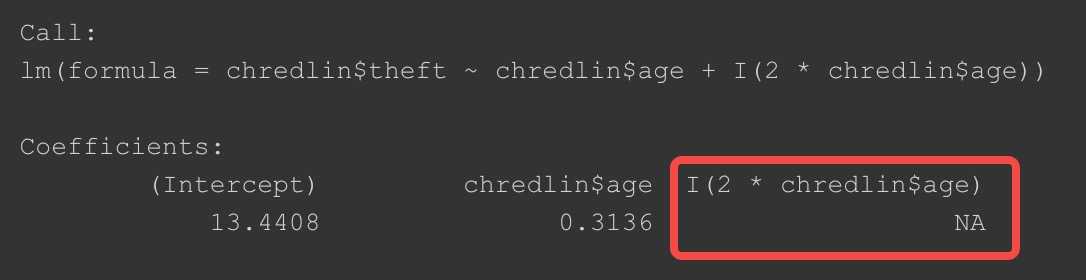
\includegraphics[width=0.8\textwidth]{Figure 4.jpeg}
        \caption{\label{fig:fig4}Screenshot showing the problem of the model 3}
    \end{figure}
    The reason this problem occurs is that the variable \textit{$2$age} is not independent to the other explanatory variable \textit{age}. This reduce the rank of the column space made by the data for the explanatory variables from $2$ to $1$. Hence, we would not have the estimate for the variable \textit{$2$age}. I plotted model $3$ on the scatter plot I made in the question $3$ together with model $1$, and I got the results below as shown in the Figure \ref{fig:fig5}.
    \begin{figure}[H]
        \centering
        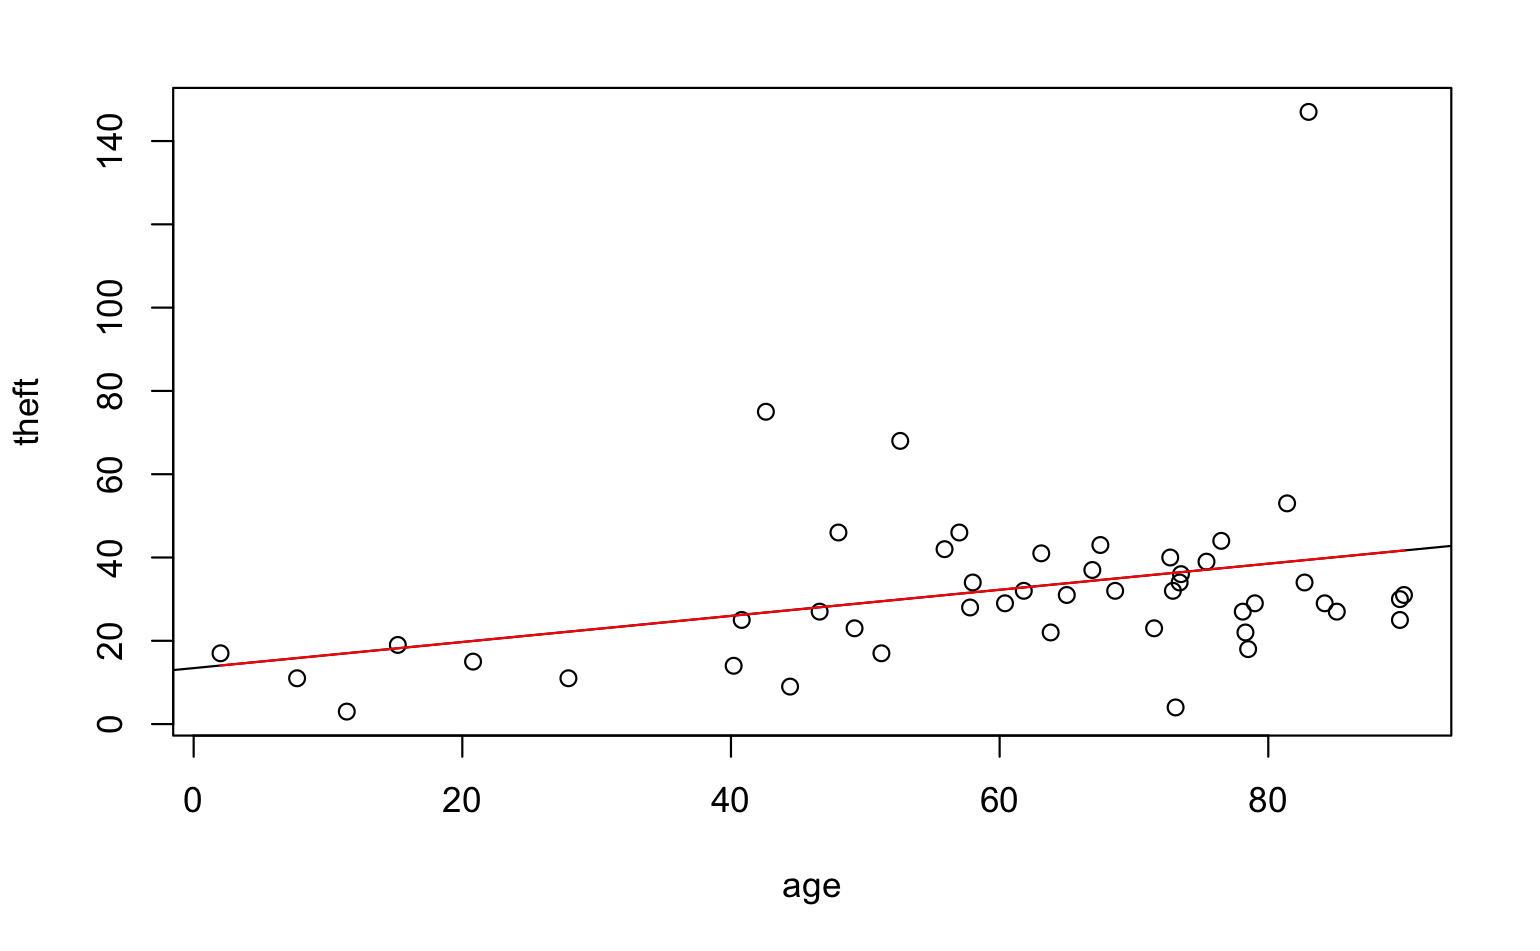
\includegraphics[width=0.8\textwidth]{Figure 5.png}
        \caption{\label{fig:fig5}Scatter plot of theft against age with model 1 and 3}
    \end{figure}
    Since the two models overlap, the model $3$ gives the same prediction as the first one.
\end{answer}
